
\section{Solutions for ``Group Actions''}
\noindent\textbf{\textit{ (Chapter \ref{actions}})}\bigskip

\noindent(\emph{NOTE that in the problems that ask to give rotations, the listings are not exhaustive: other answers are possible.})

\noindent\textbf{Exercise \ref{exercise:actions:Cube1}}
\begin{enumerate}[(a)]
\item
%Give rotations that take the bottom face ($z_-$) to each of the faces $x_-,x_+,y_-,y_+$.
	\begin{multicols}{4}
	\begin{itemize}
	\item
	$z_-\rightarrow x_-$: 
		\begin{itemize}
		\item
		$r_y$
		
		\item
		$r_y^{-3} $ 
		\end{itemize}
				
	\item
	$z_-\rightarrow x_+$: 
		\begin{itemize}
		\item
		$r_y\compose r_z^2$
		
		\item
		$r_y^{-1}$
		
		\item
		$r_y^3$
		\end{itemize}
				
	\item
	$z_-\rightarrow y_-$: 
		\begin{itemize}
		\item
		$r_x^3$
		
		\item
		$r_x^{-1}$
		\end{itemize}
				
	\item
	$z_-\rightarrow y_+$:
		\begin{itemize}
		\item
		$r_x$
		
		\item
		$r_x^{-3}$
		\end{itemize}
				
	\end{itemize}
	\end{multicols}
	
\item
%Give rotations that take the face $y_- $ to each of the faces $x_-,x_+,y_+,z_-,z_+$.
\begin{multicols}{3}
	\begin{itemize}
	\item
	$y_-\rightarrow x_-$: 
		\begin{itemize}
		\item
		$r_z^{3}$
		
		\item
		$r_x^{3}$
		\end{itemize}
				
	\item
	$y_-\rightarrow x_+$:
		\begin{itemize}
		\item
		$r_z$
		
		\item
		$r_z^{-3}$
		\end{itemize}
				
	\item
	$y_-\rightarrow y_+$:   
		\begin{itemize}
		\item
		$r_z^{-2}$ 
		
		\item
		$r_z^{2}$
		\end{itemize}
	
	\columnbreak
	
	\item
	$y_-\rightarrow z_-$:    
		\begin{itemize}
		\item
		$r_x$
		
		\item
		$r_x^{-3}$
		\end{itemize}
		
	\item
	 $y_-\rightarrow z_+$
		\begin{itemize}
		\item
		$r_x^{-1}$
		
		\item
		$r_x^{3}$
		\end{itemize}
	\end{itemize}
	\end{multicols}
	
\item
%Let's define a notation for the cube's vertices as follows.  For example, $+++$ represents the vertex in the first octant ($x>0,y>0,z>0$).  The vertex $+-\,-$ will be in the octant where $x>0,y<0,z<0$ (Which is the vertex at lower left in Figure~\ref{fig:CubeRot}).  Give rotations that take the vertex $+-\,-$ to each of the of the vertices 
%\[ +++, ~-\,++,~+\,-\,+,~ ++\,-,~-\,-\,+,~-\,+\,-,~-\,-\,-. \]
\begin{multicols}{3}
	\begin{itemize}
	\item
	$+-\,-\rightarrow +++$: 
		\begin{itemize}
		\item
		$r_x^2$
		
		\item
		$r_x^{-2}$
		\end{itemize}
 
 	\item
 	$+-\,-\rightarrow -\,++$: 
 		\begin{itemize}
 		\item
 		$r_z \circ r_x^{2}$
 		\end{itemize}
 		
 	\item
 	$+-\,-\rightarrow +-\,+$:
 		\begin{itemize}
		\item
 		$r_x^3$
 		\end{itemize}
 	
 	\item
 	$+-\,-\rightarrow ++-\,$:
 		\begin{itemize}
 		\item
 		$r_x$
 		\end{itemize}
 		
 	\item
 	$+-\,-\rightarrow -\,-\,+$:
 		\begin{itemize}
 		\item
 		$r_y^2$
 		\end{itemize}
 	
 	\item
 	$+-\,-\rightarrow -\,+-\,$:
 		\begin{itemize}
 		\item
 		$r_z^2$
 		\end{itemize}
 	\end{itemize}
	\end{multicols}
	
\item 
%Let's denote the edges of the cube as follows.  For example, $\overline{x_+,z_-}$ represents the edge where the faces $x_+$ and $z_-$ meet.  The edge $\overline{x_+,y_-}$ is where the faces $x_+$ and $y_-$ meet.  (This is the left, front-facing edge of cube in Figure~\ref{fig:CubeRot}.)  
	\begin{enumerate}[(i)]
	\item 
%	Using the above notation, list all edges of the cube.
		\begin{multicols}{4}
		\begin{itemize}
		\item
		$\overline{x_+y_+}$
		
		\item
		$\overline{x_+y_-\,}$
		
		\item
		$\overline{x_+z_+}$
		
		\item
		$\overline{x_+z_-\,}$
		
		\item
		$\overline{x_-\,y_+}$
		
		\item
		$\overline{x_-\,y_-\,}$
		
		\item
		$\overline{x_-\,z_+}$
		
		\item
		$\overline{x_-\,z_-\,}$
		
		\item
		$\overline{y_+z_+}$
		
		\item
		$\overline{y_+z_-\,}$
		
		\item
		$\overline{y_-\,z_+}$
		
		\item
		$\overline{y_-\,z_-\,}$
		\end{itemize}
		\end{multicols}
	
	
\item 
%Give rotations that take the edge $\overline{x_+y_+}$ to each of the other edges. 
	\begin{multicols}{3}
		\begin{itemize}
		\item
		$\overline{x_+y_+} \rightarrow \overline{x_+y_+}$: 
			\begin{itemize}
			\item
			\var{id}
			\end{itemize}
	 
	 	\item
	 	$\overline{x_+y_+} \rightarrow \overline{x_+y_-\,}$: 
	 		\begin{itemize}
	 		\item
	 		$r_x^2$
	 		
	 		\item
	 		$r_z^3$
	 		\end{itemize}
	 	
	 	\item
	 	$\overline{x_+y_+} \rightarrow \overline{x_+z_+}$: 
	 		\begin{itemize}
	 		\item
	 		$r_x$
	 		\end{itemize}
	 		
	 	\item
	 	$\overline{x_+y_+} \rightarrow \overline{x_+z_-\,}$: 
	 		\begin{itemize}
	 		\item
	 		$r_x^3$
	 		\end{itemize}
	 		
	 	\item
	 	$\overline{x_+y_+} \rightarrow \overline{x_-\,y_+}$: 
	 		\begin{itemize}
	 		\item
	 		$r_z$
	 		
	 		\item
	 		$r_y^2$
	 		\end{itemize}
	 		
	 	\item
	 	$\overline{x_+y_+} \rightarrow \overline{x_-\,y_-\,}$: 
	 		\begin{itemize}
	 		\item
	 		$r_z^2$
	 		\end{itemize}
	 	
	 \item
	 	$\overline{x_+y_+} \rightarrow \overline{x_-\,z_+}$: 
	 		\begin{itemize}
	 		\item
	 		$r_z \circ r_x$
	 		\end{itemize}
	 		
	 	\item
	 	$\overline{x_+y_+} \rightarrow \overline{x_-\,z_-\,}$: 
	 		\begin{itemize}
	 		\item
	 		$r_z \circ r_x^3$
	 		\end{itemize}
	 		
	 	\item
	 	$\overline{x_+y_+} \rightarrow \overline{y_+z_+}$: 
	 		\begin{itemize}
	 		\item
	 		$r_y^3$
	 		\end{itemize}
	 		
	 	\item
	 	$\overline{x_+y_+} \rightarrow \overline{y_+z_-\,}$: 
	 		\begin{itemize}
	 		\item
	 		$r_y$
	 		\end{itemize}
	 		
	 	\item
	 	$\overline{x_+y_+} \rightarrow \overline{y_-\,z_+}$: 
	 		\begin{itemize}
	 		\item
	 		$r_z^2 \circ r_y$
	 		\end{itemize}
	 		
	 	\item
	 	$\overline{x_+y_+} \rightarrow \overline{y_-\,z_-\,}$: 
	 		\begin{itemize}
	 		\item
	 		$r_z^2 \circ r_y^3$
	 		\end{itemize}
	 		
	 	\end{itemize}
		\end{multicols}

\end {enumerate}
\end{enumerate}

\noindent\textbf{Exercise \ref{exercise:actions:Cube2}}
%\\
%Consider the edge $\overline{y_+,z_+}$ of a cube.  What is the equivalence class of this edge under $G$-equivalence, where $G$ is the group of rotational symmetries of a cube? \emph{Explain} your answer.
%\\
\\
All edges of the cube are in the equivalence class.  This is due to the nature of the $G$-class, the edge $\overline{y_+z_+}$ will map to every other edge in the cube with some $g \in G$.
\\

\noindent\textbf{Exercise \ref{exercise:actions:orbits2}}
\begin{enumerate}[(a)]
\item 
%Let $G=\{\var{id},\mu_1\}$ which is a subgroup of $S_3$ (the symmetry group of an equilateral triangle) (See Figure~\ref{groups_s3_symmetry_fig} in Section~\ref{SymmetryGroup}.) Let $X=\{A,B,C\}$ be the set of vertices of an equilateral triangle. List the orbits of $X$ under $G$
%\\
%\\
The orbit of $X$ is $\{A\}, \{B, C\}$

\item 
%Let $G$ be the permutation group defined by
%\begin{align*}
%G =&\{(1), (1358),(15)(38), (1853), (247),(274), (1358)(247),(15)(38)(247),\\
%&~~ (1853)(247),(1358)(274),(15)(38)(274),(1853)(274) \}
%\end{align*}
%and $X = \{ 1, 2, 3, 4, 5,6,7,8\}$. Then $X$ is a $G$-set.  List the orbits of $X$ under $G$.
%\\
%\\
The orbits of $X$ are $\{1, 3, 5, 8\}, \{6\}, \{2, 4, 7\}$
\end{enumerate}

\noindent\textbf{Exercise \ref{exercise:actions:s4_gset_group}}
%Let $G = S_4$ (the permutations of 4 elements), and let $X = \{1,2,3,4\}$.  $X$ is a $G$-set.
\begin{enumerate}[(a)]
\item
%Give $G_2$, $G_4$, and $G_2 \cap G_4$.  Is $G_2 \cap G_4$ a group? \emph{Explain} your answer.
	\begin{itemize}
	\item
	$G_2 = \{(1), (13), (14), (34), (134), (143)\}$
	
	\item
	$G_4 = \{(1), (12), (13), (23), (123), (132)\}$
	
	\item
	$G_2 \cap G_4 = \{(1), (13)\}$
	
	\item
	Closure: $(1)(1) = (1); (1)(13) = (13); (13)(1) = (13); (13)(13) = (1)$. We have shown closure.
	\\
	Inverse: $(1)(1) = (1)(1) = (1)$ and $(13)(13) = (13)(13) = (1)$. We have shown inverse.
	\\
	So $G_2 \cap G_4$ is a group.
	\end{itemize}
	
\item
%Give $X_{(123)}$, $X_{(234)}$,and  $X_{(123)} \cap X_{(234)}$.
	\begin{itemize}
	\item
	$X_{(123)} = \{4\}$
	
	\item
	$X_{(234)} = \{1\}$
	
	\item
	$X_{(123)} \cap X_{(234)} = \O$
	\end{itemize}
	
\item
%Repeat part (a) with $G=A_4$ (the group of even permutations on 4 elements).
	\begin{itemize}
	\item
	$G_2 = \{(1), (134), (143)\}$
	
	\item
	$G_4 = \{(1), (123), (132)\}$
	
	\item
	$G_2 \cap G_4 = \{(1)\}$
	
	\item
	In Exercise \ref{exercise:Groups:trivial} we showed that the trivial group is a group, so $G_2 \cap G_4$ is a group containing only the identity element.
	\end{itemize}
	
\item
%Repeat part (b) with $G=A_4$ (the group of even permutations on 4 elements).
	\begin{itemize}
	\item
	$X_{(123)} = \{4\}$
	
	\item
	$X_{(234)} = \{1\}$
	
	\item
	$X_{(123)} \cap X_{(234)} = \O$
	\end{itemize}
\end{enumerate}

\noindent\textbf{Exercise \ref{exercise:actions:sn_gset_group}}
%Let $G = S_n$ (the permutations of n elements), and let $X = \{1,2,\ldots n \}$.  $X$ is a $G$-set.
\begin{enumerate}[(a)]
\item
%What is $|G_1|$? What is $|G_2|$? What is $|G_k|$ where $k \in X$?  (Recall that $|S_n| = n!$)
	\begin{itemize}
	\item
	$|G_1| = (n - 1)!$
	
	\item
	$|G_2| = (n - 1)!$
	
	\item
	$|G_k| = (n - 1)!$
	\end{itemize}
	
\item
%If $g$ is a $3$-cycle, then what is $|X_g|$? What if $g$  is a 5-cycle?  (You may assume that $n \ge 5$).
	\begin{itemize}
	\item
	$|X_3| = n - 3$
	
	\item
	$|X_5| = n - 5$
	\end{itemize}
	
\item
%Give a general formula for $|X_g|$, where $g$ is a $k$-cycle ($2 \le k \le n$).

$|X_g| = n - k$

\skipitems{3}
\end{enumerate}

\noindent\textbf{Exercise \ref{exercise:actions:CountingFormula2}}
\begin{enumerate}[(a)]
\item 
%Find the stabilizer subgroup for the edge $\overline{x_+,z_+}$. 
%\hyperref[sec:actions:hints]{(*Hint*)}
$G_{\overline{x_+,z_+}}=$
	\begin{itemize}
	\item
	$\{r_x^2\compose r_y, \var{id}\}$
	
	\item
	$\{r_y\circ r_z^2, \var{id}\}$
	\end{itemize}
	
\item 
%Find the stabilizer subgroup for the edge $\overline{x_-,y_+}$.
$G_{\overline{x_-,y_+}}=$
	\begin{itemize}
	\item
	$\{r_y^2\compose r_z^{-1}, \var{id}\}$
	
	\item
	$\{r_z\circ r_y^{2}, \var{id}\}$
	\end{itemize}
	
\item 
%In Example ~\ref{example:actions:CountingFormula1} we constructed a formula for $|G|$ in terms of $| G_{x_+}|$ and $|{\cal O}_{x_+}|$.  Construct a similar formula using $G_{\overline{x_+,z_+}}$ and $|{\cal O}_{\overline{x_+,z_+}}|$, and show that you get the same answer. Do the same thing with $G_{\overline{x_-,y_+}}$ and $|{\cal O}_{\overline{x_-,y_+}}|$.  
	\begin{itemize}
	\item
	$|G| = |G_{\overline{x_+,z_+}}| \cdot |{\cal O}_{\overline{x_+,z_+}}| = 24$
	
	\item
	$|G| = |G_{\overline{x_+,y_+}}| \cdot |{\cal O}_{\overline{x_+,y_+}}| = 24$
	\end{itemize}
	
\item 
%Find the stabilizer subgroup for the vertex $+,+,+$ 
%\hyperref[sec:actions:hints]{(*Hint*)}
$G_{+,+,+}=$
	\begin{itemize}
	\item
	$\{\var{id}, r_y\compose r_z, r_z^{-1}\compose r_y^{-1} \}$
	
	\item
	$\{\var{id}, r_y\circ r_z, r_x\circ r_y \}$
	\end{itemize}
	
\item 
%Find the stabilizer subgroup for the vertex $+\,,-\,,+$. 
$G_{+\,-\,+}=$
	\begin{itemize}
	\item
	$\{\var{id}, r_y\compose r_z^{-1}, r_z\compose r_y^{-1} \}$
	
	\item
	$\{\var{id}, r_x\circ r_z, r_y\circ r_z^{3}\}$
	\end{itemize}
	
\item
% Using parts (d) and (e), construct alternative formulas for $|G|$.
	\begin{itemize}
	\item
	$|G| = |G_{+,+,+}| \cdot |{\cal O}_{+,+,+}| = 24$
	
	\item
	$|G| = |G_{+\,-\,+}| \cdot |{\cal O}_{+\,-\,+}| = 24$
	\end{itemize}
\end{enumerate}

\noindent\textbf{Exercise \ref{exercise:actions:Stabilizers1}}
%Consider the edges of a cube.
\begin{enumerate}[(a)]
\item
%For each edge, how many rotations (besides the identity) leave that edge fixed?
Two faces meet at each edge so besides the identity there is 1 rotation (which switches the 2 faces)  that leaves each edge fixed.  
 
\item
%What are the orders of the rotations (besides the identity) that leave an edge fixed?
order 2 

\item
%Do edges come in pairs or not?  If so give the pairs, if not, explain why not.
Yes, each edge has another edge that is directly opposite.
	\begin{multicols}{2}
	\begin{itemize}
	\item
	 $\overline{x_+,y_+}$ and $\overline{x_-\,,y_-\,}$
	 
	\item
	 $\overline{x_+,z_+}$ and $\overline{x_-\,,z_-\,}$
	 
	 \item
	 $\overline{x_-\,,y_+}$ and $\overline{x_+,y_-\,}$
	 
	\item
	 $\overline{x_-\,,z_+}$ and $\overline{x_+,z_-\,}$
	 
	 \item
	 $\overline{y_+,z_+}$ and $\overline{y_-\,,z_-\,}$
	 
	 \item
	 $\overline{y_-,z_+}$ and $\overline{y_+,z_-\,}$
	\end{itemize}
	\end{multicols}
	
\item
%Altogether how many group elements (besides the identity) stabilize at least one edge?
There are 6 pairs of edges each stabilized by one element of order two as well as the identity.  There are 6 group elements in the stabilizers of the different edges.
\\
We obtain 1 additional element from the stabilizers of different edges.  They have an order of 2.
\end{enumerate}

\noindent\textbf{Exercise \ref{exercise:actions:Stabilizers2}}
%Based on the information given in the preceding discussion, complete the following table to characterize the group elements of the rotational symmetries of a cube according to their orders and fixed point sets (you may also find this video to be helpful: \url{http://www.youtube.com/watch?v=gBg4-lJ19Gg}).
%\hyperref[sec:actions:hints]{(*Hint*)}
\begin{center}
\begin{tabular}{ |l |c|c| r |}\hline
  Number of elements & order of the element & Type of set that it stabilizes \\ \hline
  1 & 1 & entire cube (identity) \\ \hline
  6 & 4 & face \\ \hline
 3 & 2 & face \\ \hline
8 & 3& vertex \\ \hline
6& 2 & edge \\ \hline
\end{tabular}
\end{center}

\noindent\textbf{Exercise \ref{exercise:actions:Tetra 1}}
\begin{enumerate}[(a)]
\item 
%How many degrees does $ r_{Aa}$ rotate face $a$?
120 degrees
\item 
%What is the order of $r_{Aa}$?
order 3
\end{enumerate}

\noindent\textbf{Exercise \ref{exercise:actions:Tetra4}}
%Consider the vertex $A$ of a tetrahedron.  What is the equivalence class of this vertex under $G$-equivalence, where $G$ is the groups of rotational symmetries of a tetrahedron?   (Note:  This $G$-equivalence class is the same as orbit of $A$. which we denote as ${\cal O}_A$.)
\\
$ \cal{O}_A =\{A,B,C,D\}$
\\

\noindent\textbf{Exercise \ref{exercise:actions:Tetra5}}
%Let $G$ be the rotational symmetries of a tetrahedron
\begin{enumerate}[(a)]
\item
%What is the fixed point set of $r_{Bb}$?
$X_{r_{Bb}}=\{B,b\}$

\item 
%What is the fixed point set of $r_{Bb}\compose r_{Dd}$? 
%\hyperref[sec:actions:hints]{(*Hint*)}
$X_{ r_{Bb}\compose r_{Db }}=\{A,a\}$

\skipitems{2}
\end{enumerate}

\noindent\textbf{Exercise \ref{exercise:actions:Tetra9}}
%Complete the following table (similar to the table in Exercise~\ref{exercise:actions:Stabilizers2})to characterize the group elements of the rotational symmetries of a tetrahedron according to the type(s) of sets they stabilize.  We show two rows: fill in the blanks, and add as many rows as necessary to complete the table.
%  
%\begin{tabular}{| c |c|c| r |} \hline
% \textbf{ Number of group elements} & \textbf{Order} & \textbf{Fixed point set} \\ \hline
%  1&  --& entire tetrahedron (identity) \\ \hline
%  -- & 3& vertex + face \\   
%\end{tabular}
\\
\begin{tabular}{| c |c|c| r |} \hline
\textbf{ Number of group elements} & \textbf{Order} & \textbf{Fixed point set} \\ \hline
 1&  1& entire tetrahedron (identity) \\ \hline
8 & 3 & face and vertex \\ \hline
 3 & 2 & edge \\ \hline
\end{tabular}
 \\

\noindent\textbf{Exercise \ref{exercise:actions:Octa1}}
\begin{enumerate}[(a)]
\item
% List all the faces of the octahedron using the notation above.
\begin{multicols}{4}
	\begin{itemize}
	\item
	$\triangle_{ +++}$
	
	\item
	$\triangle_{ +-\,+}$
	
	\item
	$\triangle_{ ++-\,}$
	
	\item
	$\triangle_{ +-\,-\,}$
	
	\item
	$\triangle_{-\,++}$
	
	\item
	$\triangle_{-\,-\,+}$
	
	\item
	$\triangle_{-\,+-\,}$
	
	\item
	$\triangle_{-\,-\,-\,}$
	\end{itemize}
	\end{multicols}
	
\item
% Based on Figure~\ref{fig:OctaRot}  how many faces does an octahedron have? How many vertices?  How many edges?
8 faces, 12 edges, 6 vertices
\end{enumerate}

\noindent\textbf{Exercise \ref{exercise:actions:Octa2}}
%What is the order of $r_z$?
\\
$|r_z|=4$
\\

\noindent\textbf{Exercise \ref{exercise:actions:Octa3}}
\begin{enumerate}[(a)]
\item
% Give rotations that take $\triangle _{+++}$ to each to each of the other faces.
	\begin{multicols}{2}
	\begin{itemize}
	\item
	$\triangle_{ +++} \rightarrow \triangle_{ +++}:$
		\begin{itemize}
		\item
		$\var{id}$
		\end{itemize}
		
	\item
	$\triangle_{ +++} \rightarrow \triangle_{ +-\,+}: $
		\begin{itemize}
		\item
		$r_z^3$
		\end{itemize}
	
	\item
	$\triangle_{ +++} \rightarrow \triangle_{ ++-\,}:$
		\begin{itemize}
		\item
		$r_z \circ r_x^2$
		
		\item
		$r_z^3 \circ r_x^2$
		
		\item
		$r_y$
		\end{itemize}
	
	\item
	$\triangle_{ +++} \rightarrow \triangle_{ +-\,-\,}: $
		\begin{itemize}
		\item
		$r_x^2$
		
		\item
		$r_y^3 \circ r_z$
		\end{itemize}
		
	\item
	$\triangle_{ +++} \rightarrow \triangle_{-\,++}:$ 
		\begin{itemize}
		\item
		$r_z $
		\end{itemize}
		
	\item
	$\triangle_{ +++} \rightarrow \triangle_{-\,-\,+}:$ 
		\begin{itemize}
		\item
		$r_z^2$
		\end{itemize}
		
	\item
	$\triangle_{ +++} \rightarrow \triangle_{-\,+-\,}:$
		\begin{itemize}
		\item
		$r_z^2 \circ r_x^2$
		
		\item
		$r_y^2$
		\end{itemize}
		
	\item
	$\triangle_{ +++} \rightarrow \triangle_{-\,-\,-\,}:$
		\begin{itemize}
		\item
		$r_z \circ r_x^2$
		
		\item
		$r_z^3 \circ r_x^2$
		
		\item
		$r_y^2 \circ r_z$
		\end{itemize}
	\end{itemize}
	\end{multicols}
	
\item
% Give rotations that take  $x_-$ to each of the other vertices.
	\begin{multicols}{3}
	\begin{itemize}
	\item
	$x_-\, \rightarrow x_-\: \var{id}$
	
	\item
	$x_-\, \rightarrow x_+: r_z^2$
	
	\item
	$x_-\, \rightarrow y_+: r_z^3$
	
	\item
	$x_-\, \rightarrow y_-\,: r_z$
	
	\item
	$x_-\, \rightarrow z_+: r_y $
	
	\item
	$x_-\, \rightarrow z_-\,: r_y^3$
	\end{itemize}
	\end{multicols}
	
\item
% Give a rotation that takes edge $\overline{z_+y_+}$ to each of the other edges.
	\begin{multicols}{2}
	\begin{itemize}
	\item
	$\overline{z_+y_+} \rightarrow \overline{z_+y_+}: \var{id}$
	
	\item
	$\overline{z_+y_+} \rightarrow \overline{z_+x_-\,}: r_z$
	
	\item
	$\overline{z_+y_+} \rightarrow \overline{z_+y_-\,}: r_z^2$
	
	\item
	$\overline{z_+y_+} \rightarrow \overline{z_+x_+}: r_z^3$
	
	\item
	$\overline{z_+y_+} \rightarrow \overline{x_+y_+}: r_y$
	
	\item
	$\overline{z_+y_+} \rightarrow \overline{x_-\,y_+}: r_z \circ r_y$
	
	\item
	$\overline{z_+y_+} \rightarrow \overline{x_-\,y_-\,}: r_z^2 \circ r_y$
	
	\item
	$\overline{z_+y_+} \rightarrow \overline{x_+y_-\,}: r_z^3 \circ r_y$
	
	\item
	$\overline{z_+y_+} \rightarrow \overline{y_+z_-\,}: r_y^2$
	
	\item
	$\overline{z_+y_+} \rightarrow \overline{x_-\,z_-\,}: r_z \circ r_y^2$
	
	\item
	$\overline{z_+y_+} \rightarrow \overline{y_-\,z_-\,}: r_z^2 \circ r_y^2$
	
	\item
	$\overline{z_+y_+} \rightarrow \overline{x_+z_-\,}: r_z^3 \circ r_y^2$
	\end{itemize}
	\end{multicols}
\end{enumerate}

\noindent\textbf{Exercise \ref{exercise:actions:Octa4}}
%Consider the edge $\overline{x_-y_+}$ of a octahedron. What is ${\cal O}_{\overline{x_-y_+}}$?
\\
${\cal O}_{\overline{x_-y_+}} = \{\text{all edges of the octahedron}\} = 12$
\\

\noindent\textbf{Exercise \ref{exercise:actions:Octa5}}
%Let $G$ be the rotational symmetries of an octahedron
\begin{enumerate}[(a)]
\item 
% What is the fixed point set of $r_{y}\compose r_{z}$?
$X_{r_{y}\circ r_{z}}= \{\triangle_{ +++}, \triangle_{-\,-\,-\,}\}$

\item 
%What is the fixed point set of $r_{y}^2\compose r_{x}$? 
$X_{r_{y}^2\circ r_{x}}=\{\overline {y_+z_-\,},\overline{y_-\,z_+}\}$

\item
% What is the fixed point set of $r_{x}^2\compose r_{y}$?
$X_{r_{x}^2\circ r_{y}}=\{\overline {x_+z_+},\overline{x_-\,z_-\,}\}$ 
\end{enumerate}

\noindent\textbf{Exercise \ref{exercise:actions:Octa5a}}
%Find the stabilizer subgroups for each of the vertices of the octahedron. 
%\hyperref[sec:actions:hints]{(*Hint*)}
\\
\bigskip
$G_{x_+} = G_{x_-\,} = \{\var{id}, r_x, r_x^2, r_x^3\}$
\\
\bigskip
$G_{y_+} = G_{y_-\,} = \{\var{id}, r_y, r_y^2, r_y^3\}$
\\
$G_{z_+} = G_{z_-\,} = \{\var{id}, r_z, r_z^2, r_z^3\}$
\\

\noindent\textbf{Exercise \ref{exercise:actions:Octa6}}
%Let $G$ be the rotational symmetries of an octahedron. Construct a formula for $|G|$ in terms of $| G_{y_+}|$ and $|{\cal O}_{y_+}|$ (see Example~\ref{example:actions:CountingFormula1}).
\\
$|G| = | G_{y_+}| \cdot |{\cal O}_{y_+}| = 24$
\\

\noindent\textbf{Exercise \ref{exercise:actions:Octa7}}
\begin{enumerate}[(a)]
\item
% Find the stabilizer subgroup for the edge $\overline{y_+~z_+}$. 
$G_{\overline{y_+z_+}} =$
	\begin{itemize}
	\item
	$\{\var{id}, r_z^2 \circ r_x\}$
	
	\item
	$\{\var{id}, r_x \circ r_y^2\}$
	\end{itemize}
	
\item
% Find the stabilizer subgroup for the edge $\overline{y_-~z_-}$.
$G_{\overline{y_-\,z_-\,}} =$
	\begin{itemize}
	\item
	$\{\var{id}, r_z^2 \circ r_x^2\}$
	
	\item
	$\{\var{id}, r_x \circ r_y^2\}$
	\end{itemize}
	
\item
% How many different group elements (besides the identity) stabilize at least one edge?
6, one group element stabilizes each pair of edges and there are 6 pairs of edges
\end{enumerate}

\noindent\textbf{Exercise \ref{exercise:actions:Octa8}}
\begin{enumerate}[(a)]
\item 
%Find the stabilizer subgroup for the face $\triangle_{+ + +}$.
$G_{\triangle_{+ + +}} =$
	\begin{itemize}
	\item
	$\{\var{id}, r_z \circ r_x, r_y \circ r_z\}$
	
	\item
	$\{\var{id}, r_y \circ r_z, r_y \circ r_z \circ r_y \circ r_z\}$
	\end{itemize}
	
\item 
%Find the stabilizer subgroup for the face $\triangle_{ -~-~-}$.
$G_{\triangle_{ -~-~-}} =$
	\begin{itemize}
	\item
	$\{\var{id}, r_z \circ r_x, r_y \circ r_z\}$
	
	\item
	$\{\var{id}, r_y \circ r_z, r_y \circ r_z \circ r_y \circ r_z\}$
	\end{itemize}
	
\item 
%How many different group elements stabilize at least one face?
8
\end {enumerate}

\noindent\textbf{Exercise \ref{exercise:actions:Octa9}}
%In Exercise ~\ref{exercise:actions:Octa6} we constructed a formula for $|G|$ in terms of $|G_{y_+}|$ and $|{\cal O}_{y_+}|$. Do the same thing using $|G_{\triangle_{+ + +}}|$ and $|{\cal O}_{\triangle_{+ + +}}|$, and show that you get the same value for $|G|$.
\\
$|G| = |G_{\triangle_{+ + +}}| \cdot |{\cal O}_{\triangle_{+ + +}}| = 24$
\\


\noindent\textbf{Exercise \ref{exercise:actions:Octa10}}
%Complete the following table to characterize the group elements of the rotational symmetries of an octahedron.  We show two rows, how many more to complete the table? 
% 
%\begin{tabular}{| c |c|c| r |} \hline
% \textbf{ Number of group elements} & \textbf{Order} & \textbf{Fixed point set} \\ \hline
%  ---&  ---& entire  octahedron (identity) \\ \hline
%  --- & ---&  opposite vertices \\
%
%\end{tabular}

\begin{tabular}{| l | c | r |} \hline
\textbf{ Number of group elements} & \textbf{Order} & \textbf{Fixed point set} \\ \hline
1 & 1 & entire octahedron (identity) \\ \hline
6 & 4  & opposite vertices\\ \hline
3 & 2 & opposite vertices\\ \hline
8 & 3 & opposite faces  \\ \hline
6 & 2 & opposite edges \\ \hline
\end{tabular}
\\
\\

\noindent\textbf{Exercise \ref{exercise:actions:Dodeca2}}
\begin{enumerate}[(a)]
\item 
%What is the order of $r_{f_1}$?
order 5

\item
% Let $G$ be the rotational symmetry group of a dodecahedron.  List all rotations in the stabilizer subgroup $G_{f_1}$.  What else do they stabilize?
$G_{f_1}={\var{id},r_{f_1},r_{f_1}^2, r_{f_1}^3, r_{f_1}^4}$, $G_{f_1}$ will also stabilize the opposite (parallel) face.

\item 
%What is $|G_{f_1}|?$
$|G_{f_1}|=5$

\item 
%How many group elements in $G$ stabilize at least 1 face?
25 elements 4 rotations for each of 6 pairs of opposite faces, plus the identity.

\item
% What is $|{\cal O}_{f_1}|$?
$|{\cal O}_{f_1}|=12$ The orbit of $f_1$ includes all faces of the dodecahedron.
\end{enumerate}

\noindent\textbf{Exercise \ref{exercise:actions:Dodeca3}}
\\
$5\times 12=60$
\\

\noindent\textbf{Exercise \ref{exercise:actions:Dodeca4}}
\begin{enumerate} 
\item
% Find the order of $r_{v_1}$.
order 3

\item 
%List all rotations in the stabilizer subgroup $G_{v_1}$.  What else do they stabilize?
$G_{v_1}={\var{id},r_{v_1},r_{v_1}^2}$ $G_{v_1}$ will also stabilize the opposite vertex.

\item
% How many group elements in $G$ (besides the identity) stabilize at least 1 vertex?
20 rotations 10 pairs of vertices, 2 rotations besides the identity stabilize each pair.

\item
% What is $|{\cal O}_{v_1}|$?
$|{\cal O}_{v_1}|=20$ The orbit of $v_1$ includes all the vertices of the dodecahedron.
\end{enumerate}


\noindent\textbf{Exercise \ref{exercise:actions:Dodeca5}}
\begin{enumerate}[(a)]
\item
% Let $e_1$ be one edge of the dodecahedron. What is $|G_{e_1}|$?
2

\item 
%%Are the edges of a dodecahedron stabilized in pairs?  Explain your answer.
%\hyperref[sec:actions:hints]{(*Hint*)}
There are 60 group elements in $G$.  By previous exercise 25 elements stabilize faces, 20 rotations stabilize vertices. We need 15 more elements to make up $G$.  There are $30/2=15$ pairs of edges, so edges must come in pairs.
\end{enumerate}

\noindent\textbf{Exercise \ref{exercise:actions:Dodeca6}}
\begin{enumerate}[(a)]
\item
% How many group elements of $G$ besides the identity stabilize at least 1 edge?
15, one rotation for each pair of edges.

\item
%Complete the following table to characterize the group elements of the rotational symmetries of a dodecahedron.  We show two rows, how many more to complete the table?  
%\begin{tabular}{| c |c|c| r |} \hline
% \textbf{ Number of group elements} & \textbf{order} & \textbf{Fixed point set} \\ \hline
%  --&  --& entire  dodecahedron (identity) \\ \hline
%  -- & --&  -- \\ 
%\end{tabular}
%\end{enumerate}
\begin{tabular}{| c |c|c| r |}\hline
Number of elements & order of the element & Type of set that it stabilizes \\ \hline
1 & 1 & entire dodecahedron (identity) \\ \hline
24 & 5 & face \\ \hline
15 & 2 & edge\\ \hline
20 & 3  & vertices\\ \hline
\end{tabular}
\end{enumerate}

\noindent\textbf{Exercise \ref{exercise:actions:Soccer1}}
\begin{enumerate}[(a)]
\item
%Given one particular pentagonal face of the soccer ball, what is the order of its stabilizer?
order = 5
\item
%Given that there are 12 pentagonal faces, find $|G|$ where $G$ is  group of rotational symmetries of the soccer ball.
%\hyperref[sec:actions:hints]{(*Hint*)}
$|G| = |G_{\text{faces pentagon}} \cdot |{\cal O}_{\text{faces pentagon}}| = 60$
\end{enumerate}

\noindent\textbf{Exercise \ref{exercise:actions:Soccer2}}
\begin{enumerate}[(a)]
\item
%Given one particular hexagonal face of the soccer ball, what is the order of its stabilizer?
order = 3

\item
%Using your answers to (a) and part (b) of Exercise~\ref{exercise:actions:Soccer1}, determine the number of hexagonal faces. \hyperref[sec:actions:hints]{(*Hint*)}
$|G| = 60 \implies 60 = |G_{\text{hex faces}}| \cdot |{\cal O}_{\text{hex faces}}| \implies 60 = 3 \cdot |{\cal O}_{\text{hex faces}}| \implies 20 = |{\cal O}_{\text{hex faces}}|$
\end{enumerate}

\noindent\textbf{Exercise \ref{exercise:actions:Soccer3}}
\begin{enumerate}[(a)]
\item
%Consider an edge which joins a hexagonal face and a pentagonal face. How many rotations (besides the identity) stabilize this edge?  \emph{Explain} your answer.
There are no symmetries that stabilize an edge, because other than the id if you rotate it $180^{\circ}$ the edge will be in the correct position but the faces will be flipped.

\item
%Consider an edge which joins two hexagonal faces. How many rotations stabilize this edge?  \emph{Explain} your answer.
There are 2 rotations, the id and $180^{\circ}$.  The edge will be in the correct position and the faces are the same so they can be on either side.

\item
%Using the counting formula and your answers to previous exercises, determine the number of edges which join  two hexagons.
$|G| = |G_{\text{hex edges}}| \cdot |{\cal O}_{\text{hex edges}}| = 30$

\item
%Note each pentagon touches 5 hexagons. Use this information and information from Exercise~\ref{exercise:actions:Soccer1} to determine the number of edges which join a pentagon and hexagon.
There are 12 pentagonal faces and each one touches 5 hexagons. $5 \cdot 12 = 60$
\end{enumerate}

\noindent\textbf{Exercise \ref{exercise:actions:Soccer4}}
\begin{enumerate}[(a)]
\item
%Consider a particular vertex. How many rotations (besides the identity) stabilize this edge?  \emph{Explain} your answer.
The faces are only in the correct position for the identity rotation.

\item
%Note each vertex touches one pentagon, and each pentagon has five vertices. Use this information and information from Exercise~\ref{exercise:actions:Soccer1} to determine the number of vertices.
With 5 vertices per pentagon and 12 pentagonal faces there are 60 vertices.
\end{enumerate}

\noindent\textbf{Exercise \ref{exercise:actions:Eulers1}}
\begin{enumerate}[(a)]
\item
%Complete the table and compare $|G|$ to the number of edges of each polyhedron.  The number of edges is equal to the order of the orbit of any edge $e$, denoted as $|{\cal O}_e|$.
%
%\begin{tabular}{|c | c | c|}\hline
%polyhedron & number of edges ($|{\cal O}_e|$) & order of group ($|G|$)\\ \hline
%cube &  12 &   24\\ \hline
%tetrahedron &  -- &   --\\ \hline
%octahedron & -- &--\\ \hline
%dodecahedron &  --&--\\ \hline 
%\end{tabular}
\begin{tabular}{|c | c | c|}\hline
polyhedron & number of edges ($|{\cal O}_e|$) & order of group ($|G|$)\\ \hline
cube &  12 &   24\\ \hline
tetrahedron &  6&   12\\ \hline
octahedron & 12 &24\\ \hline
dodecahedron &  30&60\\ \hline 
\end{tabular}

\item
% Based on the table, guess an equation for $|G|$ in terms of ${\cal O}_e$.
$|G| = 2 \cdot {\cal O}_e$

\item 
%Prove your equation using Proposition~\ref{proposition:actions:CountingFormula}.
By Proposition \ref{proposition:actions:CountingFormula}, $|{\cal O}_x| = [G : G_x]$.  
\\
This can be rewritten as $|{\cal O}_x| = \frac{|G|}{|{G_x|}}$, by Definition \ref{factor_group}.
\\
By multiplication we get $|G| = |G_x| \cdot |{\cal O}_x|$. 
\\
Since the stabilization group of an edge has an order of two, (only two faces share any one edge), then $|G| = 2 \cdot |{\cal O}_e|$.
\end{enumerate}

\noindent\textbf{Exercise \ref{exercise:actions:Euler5}}
%A certain regular polyhedron has 20 triangular faces. 
\begin{enumerate}[(a)]
\item
%Using Proposition~\ref{proposition:actions:CountingFormula}, find the number of edges.
By Proposition \ref{proposition:actions:CountingFormula}, $|{\cal O}_x| = [G : G_x]$.  
\\
This can be rewritten as $|{\cal O}_x| = \frac{|G|}{|{G_x|}}$, by Definition \ref{factor_group}.
\\
By multiplication we get $|G| = |G_\text{faces}| \cdot |{\cal O}_\text{faces}|$. 
\\
$|G| = 3 \cdot 20 \implies 60$ faces
\\
$|G| = |G_\text{egdes}| \cdot |{\cal O}_\text{edges}|$
\\
$60 = 2 \cdot |{\cal O}_\text{edges}|$
\\
$30 = |{\cal O}_\text{edges}|$

\item
%Using Euler's formula, find the number of vertices.
$|{\cal O}_f| + |{\cal O}_v| - |{\cal O}_e| = 2$
\\
$20 +  |{\cal O}_v| -30 = 2$
\\
$ |{\cal O}_v| = 12$

\item
%Using Proposition~\ref{proposition:actions:CountingFormula}, find the number of edges which meet at each vertex.
$\frac{60}{12} = 5$, edges meet at one vertex.
\end{enumerate}
 
 
\noindent\textbf{Exercise \ref{exercise:actions:Euler 4}}
\begin{enumerate}[(a)]
\item 
%Verify Euler's formula for the cube and tetrahedron.
	\begin{itemize}
	\item
	Cube:
	\\
	$|{\cal O}_f| + |{\cal O}_v| - |{\cal O}_e| = 2$
	\\
	$6 + 8 -12 = 2$
	
	\item
	Tetrahedron:
	\\
	$|{\cal O}_f| + |{\cal O}_v| - |{\cal O}_e| = 2$
	\\
	$4 + 4 - 6 = 2$
	\end{itemize}
	
\item 
%Explain why the proof we have given does not apply to the soccer ball. Verify that notwithstanding, Euler's formula still works for the soccer ball anyway! 
The proof works with polyhedrons with faces, edges, and vertices of the same order.  The soccer ball's faces and edges have different orders.
\\
Verify:
\begin{align*}
(|{\cal O}_{\text{pen faces}}| + |{\cal O}_{\text{hex faces}}|) +  (|{\cal O}_{\text{vertices}}|)  -  (|{\cal O}_{\text{pen edges}}| + |{\cal O}_{\text{hex edges}}|) &= 2 
\\
[(12) + (20)] + (60) - [(60) + (30)] &= 2 
\\
92 - 90 &= 2
\\
2 &= 2 
\end{align*}
\end{enumerate}
 
\noindent\textbf{Exercise \ref{exercise:actions:Conj1}}

%For each $\sigma$ and $f$, complete a commutative diagram like the one in Figure~\ref{fig:Commutative1}. Find the conjugate mapping using the relabeling method, and verify that the result agrees with $f \compose \sigma \compose f^{-1}$.
\begin{enumerate}[(a)]
\item
% $\sigma=(12)(35)$ and $f=\begin{pmatrix} 1&2&3&4&5\\ A&B&C&D&E& \end{pmatrix} $
\begin{figure}[H]
\begin{center}
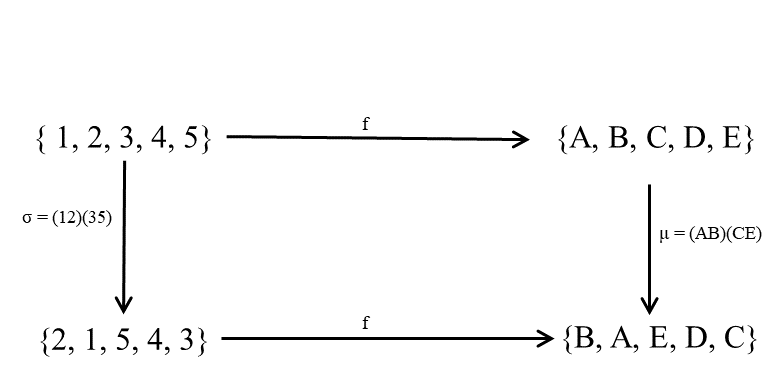
\includegraphics[width=3in]{images/Conj1a.png}
\caption{Conjugate mapping with $\sigma$ and $\mu$ permuting $\{1,2,3,4,5\}$.}
\end{center}
\end{figure}

\item
% $\sigma=(2346)$ and $f=\begin{pmatrix} 1&2&3&4&5&6\\ A&B&C&D&E&F \end{pmatrix}$
\begin{figure}[H]
\begin{center}
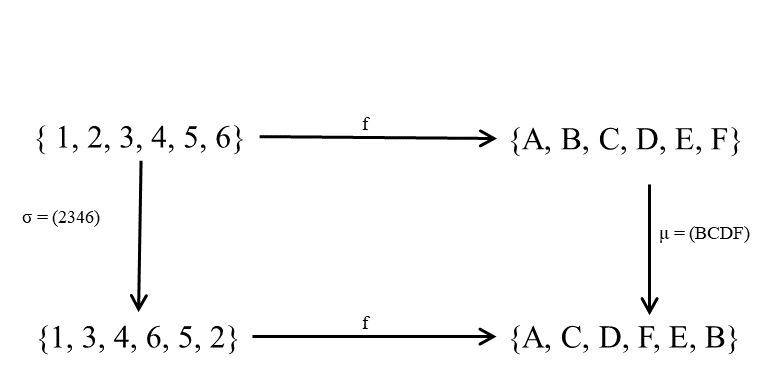
\includegraphics[width=3in]{images/Conj1b.png}
\caption{Conjugate mapping with $\sigma$ and $\mu$ permuting $\{1,2,3,4,5,6\}$.}
\end{center}
\end{figure}
\end{enumerate}

\noindent\textbf{Exercise \ref{exercise:actions:Conj3}}
%Given $\sigma$ and $\tau$ use the relabeling method to find the permutation conjugate to $\sigma$.  Check your work by computing $\tau\sigma\tau^{-1}$.
\begin{enumerate}[(a)]
\item 
%$\sigma=(6247)$ and $\tau=(527)(63)$.  $\sigma$ and $\tau$ act on the set $\{1,2,3,4,5,6,7\}$.
$\tau=\begin{pmatrix}1&2&3&4&5&6&7\\6&7&3&2&1&5&4
\end{pmatrix}$
\begin{align*}
\tau \circ \tau^{-1} &= (527)(63) \circ (6247) \circ (527)^2 (63)
\\
&= (527)(63) \circ (6247)\circ (257)(63)
\\
&= (527)(63) \circ (2563)(47)
\\
&= (3745)
\end{align*}

\item
%$\sigma=(256)(134)$ and $\tau=(21643)$.  $\sigma$ and $\tau$ act on the set $\{1,2,3,4,5,6\}$.
$\tau=\begin{pmatrix}1&2&3&4&5&6\\6&1&2&3&5&4
\end{pmatrix}$
\begin{align*}
\tau \circ \tau^{-1} &= (21643) \circ (256)(134) \circ (21643)^4
\\
&= (21643) \circ (256)(134) \circ (12346)
\\
&= (21643) \circ (1563)(24)
\\
&= (154)(236)
\end{align*}

\skipitems{1}
\end{enumerate}

\noindent\textbf{Exercise \ref{exercise:actions:Conj5}}
%In each of the following find a permutation $\tau$ that makes $\sigma$ and $\mu$ conjugate.  Check that $\sigma$ and $\mu$ are conjugate according to: $\mu = \tau \sigma \tau^{-1}$.

\begin{enumerate}[(a)]
\item
% $\sigma=(135)(792)(468)$, $\mu=(236)(189)(457)$
	\begin{multicols}{3}
	\begin{itemize}
	\item
	$1 \rightarrow 4$
	
	\item
	$2 \rightarrow 6$
	
	\item
	$3 \rightarrow 5$
	
	\item
	$4 \rightarrow 1$
	
	\item
	$5 \rightarrow 7$
	
	\item
	$6 \rightarrow 8$
	
	\item
	$7 \rightarrow 2$
	
	\item
	$8 \rightarrow 9$
	
	\item
	$9 \rightarrow 3$
	\end{itemize}
	\end{multicols}
$\tau = (14)(2689357)$
\\
check: $(14)(2689357)(135)(792)(468)(2753986)(14) = (189)(236)(457) = \mu$

\item
% $\sigma=(2879)(3561)$, $\mu=(2461)(5793)$
	\begin{multicols}{3}
	\begin{itemize}
	\item
	$1 \rightarrow 3$
	
	\item
	$2 \rightarrow 2$
	
	\item
	$3 \rightarrow 5$
	
	\item
	$4 \rightarrow 8$
	
	\item
	$5 \rightarrow 7$
	
	\item
	$6 \rightarrow 9$
	
	\item
	$7 \rightarrow 6$
	
	\item
	$8 \rightarrow 4$
	
	\item
	$9 \rightarrow 1$
	\end{itemize}
	\end{multicols}
$\tau = (135769)(48)$
\\
check: $(135769)(48)(2879)(3561)(48)(196753) = (1246)(3579) = \mu$

\skipitems{1}
\end{enumerate}

\noindent\textbf{Exercise \ref{exercise:actions:Conj7}}
%Complete the previous example with $G=D_4$ and $H=\{e,s\}$ by listing all the pairs $(h,g)$ with $h\in H$ and $g \in G$ together with the result of the mapping $hgh^{-1}$.  Simplify your expression for $hgh^{-1}$ as much as possible.
\\
$H = \{e, s\}$ and $G = \{e, r, r^2, r^3, s, s \circ r, s \circ r^2, s \circ r^3\}$
\begin{align*}
(h, g) &\implies hgh^{-1}
\\
(e, e) &\implies e \circ e \circ e^{-1} \implies e
\\
(e, r) &\implies e \circ r \circ e^{-1} \implies r
\\
(e, r^2) &\implies e \circ r^2 \circ e^{-1} \implies r^2
\\
(e, r^3) &\implies e \circ r^3 \circ e^{-1} \implies r^3
\\
(e, s) &\implies e \circ s \circ e^{-1} \implies s
\\
(e, s \circ r) &\implies e \circ s \circ r \circ e^{-1} \implies s \circ r
\\
(e, s \circ r^2) &\implies e \circ s \circ r^2 \circ e^{-1} \implies s \circ r^2
\\
(e, s \circ r^3) &\implies e \circ s \circ r^3 \circ e^{-1} \implies s \circ r^3
\\
(s, e) &\implies s \circ e \circ s^{-1} \implies e
\\
(s, r) &\implies s \circ r \circ s^{-1} \implies s \circ r \circ s \implies s \circ s \circ r^3 \implies r^3
\\
(s, r^2) &\implies s \circ r^2 \circ s^{-1} \implies s \circ r^2 \circ s \implies s \circ s \circ r^2 \implies r^2
\\
(s, r^3) &\implies s \circ r^3 \circ s^{-1} \implies s \circ r^3 \circ s \implies s \circ s \circ r \implies r
\\
(s, s) &\implies s \circ s \circ s^{-1} \implies s^2 \circ s \implies s
\\
(s, s \circ r) &\implies s \circ s \circ r \circ s^{-1} \implies r \circ s \implies s \circ r^3
\\
(s, s \circ r^2) &\implies s \circ s \circ r^2 \circ s^{-1} \implies r^2 \circ s \implies s \circ r^2
\\
(s, s \circ r^3) &\implies s \circ s \circ r^3 \circ s^{-1} \implies r^3 \circ s \implies s \circ r
\end{align*}

\noindent\textbf{Exercise \ref{exercise:actions:Conj8}}
%Fill in the blanks to prove the proposition:
%
%\noindent
%First, we have that $\underline{~<1>~}$ is in  $H$ and $e.g=\underline{~<2>~}g\underline{~<3>~} = g$.
%So the identity condition for a group action holds. 
%
%Also, observing that
%\[(h_1h_2).g =\underline{~<4>~}g\underline{~<5>~}
%= h_1(h_2g\underline{~<6>~} )\underline{~<7>~}
%= h_1. (\underline{~<8>~}. g)),\]
%we see that the compatibility condition is also satisfied.
\begin{multicols}{4}
\begin{enumerate}
\item
$e$

\item
$e$

\item
$e^{-1}$

\item
$h_1h_2$ 

\item
$(h_1h_2)^{-1}$

\item
$h_2^{-1}$

\item
$h_1^{-1}$

\item
$h_2$
\end{enumerate}
\end{multicols}

\noindent\textbf{Exercise \ref{exercise:actions:Conj15b}}
%Fill in the blanks to complete the proof that a group element and its conjugate always have the same order.
%
%Suppose that $\tilde{g}$ is conjugate to $g$. This means that there exists an $x\in G$ such that $\tilde{g}=\underline{~<1>~}$. Suppose $|g|=n$. Compute $\tilde{g}^n$ as follows:
%\begin{align*}
% \tilde{g}^n&=(\tilde{g} \ldots \tilde{g}~~~~~~~~~~~~(n~\text{ times)}\\ 
%&=(\underline{~<2>~}) \ldots (\underline{~<3>~})~~~~~~~~~~~~(n~\text{ substitutions)}\\ 
%& =xg(\underline{~<4>~})g \ldots g(\underline{~<5>~})gx^{-1}\qquad\text{(associative property)}\\
%&=xg(\underline{~<6>~})g...g(\underline{~<7>~})gx^{-1}\quad\text{( inverse property)}\\
%&=x(\underline{~<8>~})x^{-1}\quad\text{( identity property)}\\
%&=x(\underline{~<9>~})x^{-1}\quad\text{(definition of order)}\\
%&=\underline{~<10>~}\quad\text{(identity and inverse properties)}
%\end{align*}
%\noindent
%From Proposition~\ref{proposition:Groups:Cyclic_subgrp_order}, it follows that  $| \tilde{g}|$ divides $|\underline{~<11>~}|$. On the other hand, \[(\underline{~<12>~})\tilde{g}(\underline{~<13>~})=g\qquad\text{(inverse property)}.\]  
%The same proof  with $g$ and $\tilde{g}$ interchanged shows that $|g|$ divides $|\underline{~<14>~}|$ Therefore,  $|g|=\underline{~<15>~}$ 
\begin{multicols}{4}
\begin{enumerate}
\item
$xgx^{-1}$

\item
$xgx^{-1}$

\item
$xgx^{-1}$

\item
$x^{-1}x$

\item
$x^{-1}x$

\item
$e$

\item
$e$

\item
$g^n$

\item
$e$

\item
$e$

\item
$|g|$

\item
$x^{-1}$

\item
$x$

\item
$|\tilde{g}|$

\item
$|\tilde{g}|$
\end{enumerate}
\end{multicols}

\noindent\textbf{Exercise \ref{exercise:actions:Conj17}}
\begin{enumerate}[(a)]
\item
% Complete a conjugacy table like the one in  Example~\ref{example:actions:Conj16} for $G=D_4$. As in the example $r$ is a counterclockwise rotation by  $90^{\circ}$ and $s$ is the reflection that leaves the vertex labeled "1" fixed. Compute and simplify the conjugate expressions as compositions of $r$ and $s$. We show one row.  How many more rows are needed to complete the table?
%
%\begin{center}
%
%\begin{tabular}{ |r| c | c |c |c |c |c | c|c |} \hline
%  $g$ &$\var{id}$ & $r$ &$r^2$ &$r^3$ & $s$ &$s\compose r$ & $s\compose r ^2$ & $s\compose r^3$\\ \hline
%  $g\compose \var{id}\compose g^{-1}$ &--- & -- & -- &-- &--&--&--&-- \\
%\end{tabular}
%\end{center}
%
% Remember, once a group element appears in a row, you don't need to compute a row for that element, because you have already found its conjugacy class.
\begin{tabular}{ |r| c | c |c |c |c |c | c|c |} \hline
  $g$ &$\var{id}$ & $r$ &$r^2$ &$r^3$ & $s$ &$s\circ r$ & $s\circ r ^2$ & $s\circ r^3$\\ \hline
  $g\circ \var{id}\circ g^{-1}$ & $\var{id}$ & $\var{id}$ & $\var{id}$ & $\var{id}$ & $\var{id}$ & $\var{id}$ & $\var{id}$ & $\var{id}$ \\ \hline
  $g\circ r \circ g^{-1}$ & $r$ & $r$ & $r$ & $r$ & $r^3$ & $r^3$ & $r^3$ & $r^3$ \\ \hline
  $g\circ r^2 \circ g^{-1}$ & $r^2$ & $r^2$ & $r^2$ & $r^2$ & $r^2$ & $r^2$ & $r^2$ & $r^2$\\ \hline
  $g\circ s \circ g^{-1}$ & $s$ & $s \circ r^2$ & $s$ & $s \circ r^2$ & $s$ & $s \circ r^2$ & $s$ & $s \circ r^2$ \\ \hline
  $g\circ (s \circ r) \circ g^{-1}$ & $s \circ r$ & $s \circ r^3$ & $s \circ r$ & $s \circ r^3$ & $s \circ r^3$ & $s \circ r$ & $s \circ r^3$ & $s \circ r$ \\ \hline
\end{tabular}

\item 
%Verify that the class equation correctly calculates $|D_4|$.
$|D|_4| = 1 + 2 + 1 + 2 + 2 = 8$
\end{enumerate}

\noindent\textbf{Exercise \ref{exercise:actions:Conj21}}
%Let $G$ be an abelian group of finite order and $x,g\in G$.
%Simplify the conjugate expression $x\compose g\compose x^{-1}$.  How many conjugacy classes are in the abelian group $G$? How many elements are in each conjugacy class? 
\\
Since $G$ is abelian, 
\begin{align*}
x \circ g \circ x^{-1} &= x \circ x^{-1} \circ g &&\text{(commutative)}
\\
&= e \circ g &&\text{(inverse)}
\\
&= g &&\text{(identity)}
\end{align*}
The number of conjugacy classes is equal to $|G|$. There is only 1 element in each conjugacy class.
